\documentclass{article}

\usepackage[spanish]{babel}
\usepackage{mathdots}
\usepackage{listings}
\usepackage{color}
\usepackage[numbers,sort&compress]{natbib}
\usepackage{graphicx}
\usepackage{subfigure}
\usepackage{url}
\usepackage{amsmath}
\usepackage{hyperref}
\usepackage[top=15mm, bottom=40mm, left=15mm, right=15mm]{geometry}
\setlength{\parskip}{2mm}
\setlength{\parindent}{0pt}

\setlength{\parskip}{2mm}
\setlength{\parindent}{0pt}
\definecolor{blue}{rgb}{0,0.6,0}
\definecolor{gray}{rgb}{0.3,0.3,0.3}
\definecolor{orange}{rgb}{0.8,0.4,0}
\definecolor{mostaza}{rgb}{0.9,0.8,0.1}

\lstset{ %
  language=R,                     % the language of the code
  basicstyle=\footnotesize,       % the size of the fonts that are used for the code
  numbers=left,                   % where to put the line-numbers
  numberstyle=\tiny\color{gray},  % the style that is used for the line-numbers
  stepnumber=1,                   % the step between two line-numbers. If it's 1, each line
                                  % will be numbered
  numbersep=5pt,                  % how far the line-numbers are from the code
  backgroundcolor=\color{white},  % choose the background color. You must add \usepackage{color}
  showspaces=false,               % show spaces adding particular underscores
  showstringspaces=false,         % underline spaces within strings
  showtabs=false,                 % show tabs within strings adding particular underscores
  frame=single,                   % adds a frame around the code
  rulecolor=\color{black},        % if not set, the frame-color may be changed on line-breaks within not-black text (e.g. commens (green here))
  tabsize=2,                      % sets default tabsize to 2 spaces
  captionpos=b,                   % sets the caption-position to bottom
  breaklines=true,                % sets automatic line breaking
  breakatwhitespace=false,        % sets if automatic breaks should only happen at whitespace
  title=\lstname,                 % show the filename of files included with \lstinputlisting;
                                  % also try caption instead of title
  keywordstyle=\color{orange},      % keyword style
  commentstyle=\color{blue},   % comment style
  stringstyle=\color{mostaza},      % string literal style
  escapeinside={\%*}{*)},         % if you want to add a comment within your code
  morekeywords={*,...}            % if you want to add more keywords to the set
} 

\author{1445183}
\title{Práctica 12: red neuronal}
\date{\today}

\begin{document}

\maketitle

\section{Objetivo}
Estudiar de manera sistemática el desempeño de la red neuronal para diez dígitos en función de las tres probabilidades asignadas a la generación de dígitos (\texttt{ngb}) en el código proporcionado por esta práctica \cite{elisaweb12} variando a las tres en un experimento factorial adecuado.

\section{Descripción}

El código se paraleliza desde el principio, usando tres núcleos de los cuatro posibles.

\begin{lstlisting}[language=R]
cluster <- makeCluster(detectCores() - 1)


binario <- function(d, l) {
  b <-  rep(FALSE, l)
  while (l > 0 | d > 0) {
    b[l] <- (d %% 2 == 1)
    l <- l - 1
    d <- bitwShiftR(d, 1)
  }
  return(b)
}
decimal <- function(bits, l) {
  valor <- 0
  for (pos in 1:l) {
    valor <- valor + 2^(l - pos) * bits[pos]
  }
  return(valor)
}

.
.
.

 clusterExport(cluster, c( "neuronas", "binario", "decimal", "modelos", "tope" ,"k", "dim", "n"))
        
        
        #PRUEBA 
        contadores <-parSapply(cluster, 1:prueba , function(x){ 
          d <- sample(0:tope, 1)
          pixeles <- runif(dim) < modelos[d + 1,] # fila 1 contiene el cero, etc.
          correcto <-binario(d, n)
          salida <- rep(FALSE, n)
          for (i in 1:n) {
            w <- neuronas[i,]
            deseada <- correcto[i]
            resultado <- sum(w * pixeles) >= 0
            salida[i] <- resultado
          }
          r <- min(decimal(salida, n), k) 
          return(r==d)})
        datos<-rbind(datos, data.frame(Replica= replicas, Negro=pn, Gris=pg, Blanco=pb, Porcentaje=(sum(contadores)/prueba)*100))
    
      }
    }
  }
}

\end{lstlisting}

Se genera un archivo \textit{CSV} con los datos proporcinados por la práctica para indicar la ubicación de los pixeles y se vincula al código en la rutina de generación de pixeles (\texttt{ngb}), después se varían las probabilidades para \texttt{ngb} como se muestra en el siguiente código haciendo uso de \texttt{for} con \texttt{20} repeticiones cada una y obteniendo los respectivos porcentajes para cada combinación.

\begin{lstlisting}[language=R]
#repeticiones
replica<-20

tmax<-5000
entrenamiento <- ceiling(0.7 * tmax)
prueba <- tmax - entrenamiento
datos<- data.frame( Replica= integer(), Negras=integer(), Grises=integer(), Blancas=integer(), Porcentaje=integer())


#archivo csv
modelos <- read.csv("digitos.modelo.csv", sep=" ", header=FALSE, stringsAsFactors=F)

#variar probabilidades 
for (PN in c(0.995,0.92,0.002)) {
  for(PG in c(0.92,0.002,0.995)){
    for(PB in c(0.002,0.995,0.92)){
     
      modelos[modelos=='n'] <- pn # pixeles negros en plantillas
      modelos[modelos=='g'] <- pg # pixeles grises en plantillas
      modelos[modelos=='b'] <- pb # pixeles blancos en plantillas
      for(replicas in 1:replica){
        print(replicas)
      
        tasa <- 0.15
        contadores <-vector()
        n <- floor(log(k-1, 2)) + 1
        neuronas <- matrix(runif(n * dim), nrow=n, ncol=dim) # perceptrones
       
        
         #ENTRENAMIENTO
        for (t in 1:entrenamiento) { # entrenamiento
          d <- sample(0:tope, 1)
          pixeles <- runif(dim) < modelos[d + 1,]
          correcto <- binario(d, n)
          for (i in 1:n) {
            w <- neuronas[i,]
            deseada <- correcto[i]
            resultado <- sum(w * pixeles) >= 0
            if (deseada != resultado) {
              ajuste <- tasa * (deseada - resultado)
              tasa <- tranqui * tasa
              neuronas[i,] <- w + ajuste * pixeles
            }
          }
        }
\end{lstlisting}



\newpage


\section{Resultados}
En la figura \ref{fig1}\textit{a} se puede observar que existe mayor porcentaje cuando la probabilidad de \textit{Negro} es mayor (crecano al 1).    \par
En la figura \ref{fig1}\textit{b} el mayor porcentaje es cuando la probabilidad es mayor en \textit{Gris}. \par
En la figura \ref{fig1}\textit{c} el mayor porcentaje se encuentra a cualquier probabilidad de \textit{Negro} (preferentemente cercano al 0)y mayor probabilidad de \textit{Gris}.
 

\begin{figure}[h!]
\centering
\subfigure[]{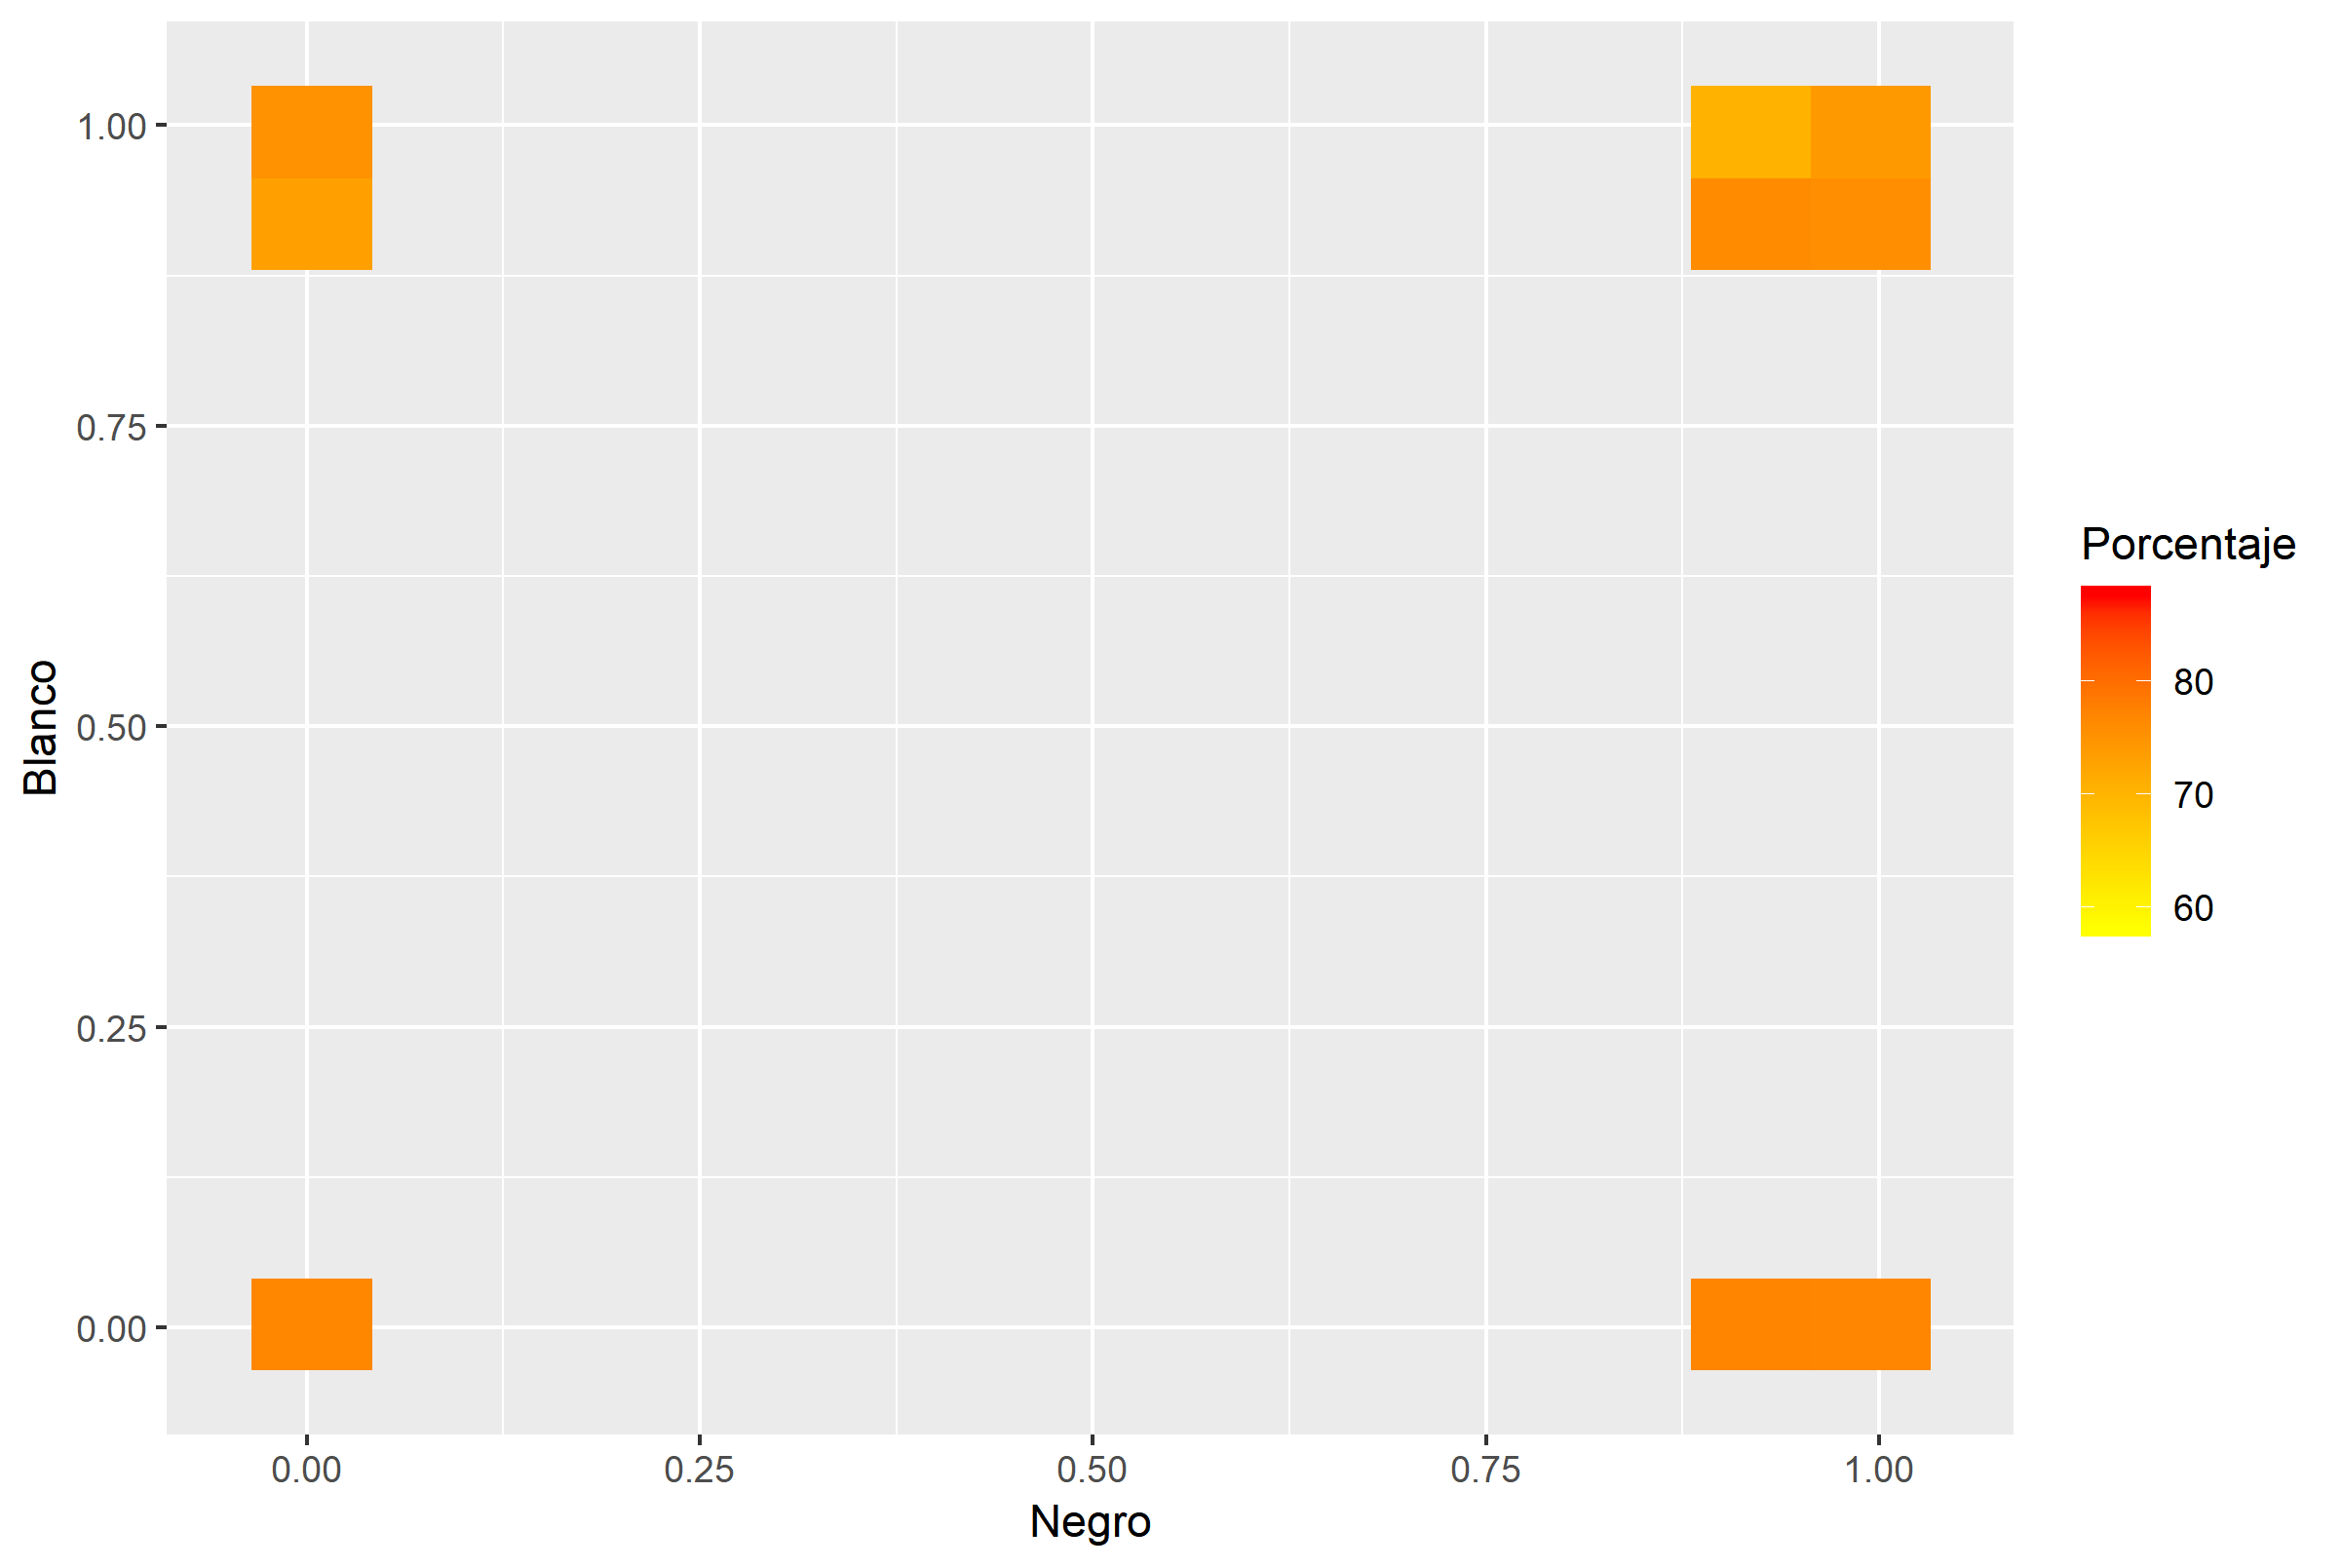
\includegraphics[width=80mm]{./plot_BN.png}}
\subfigure[]{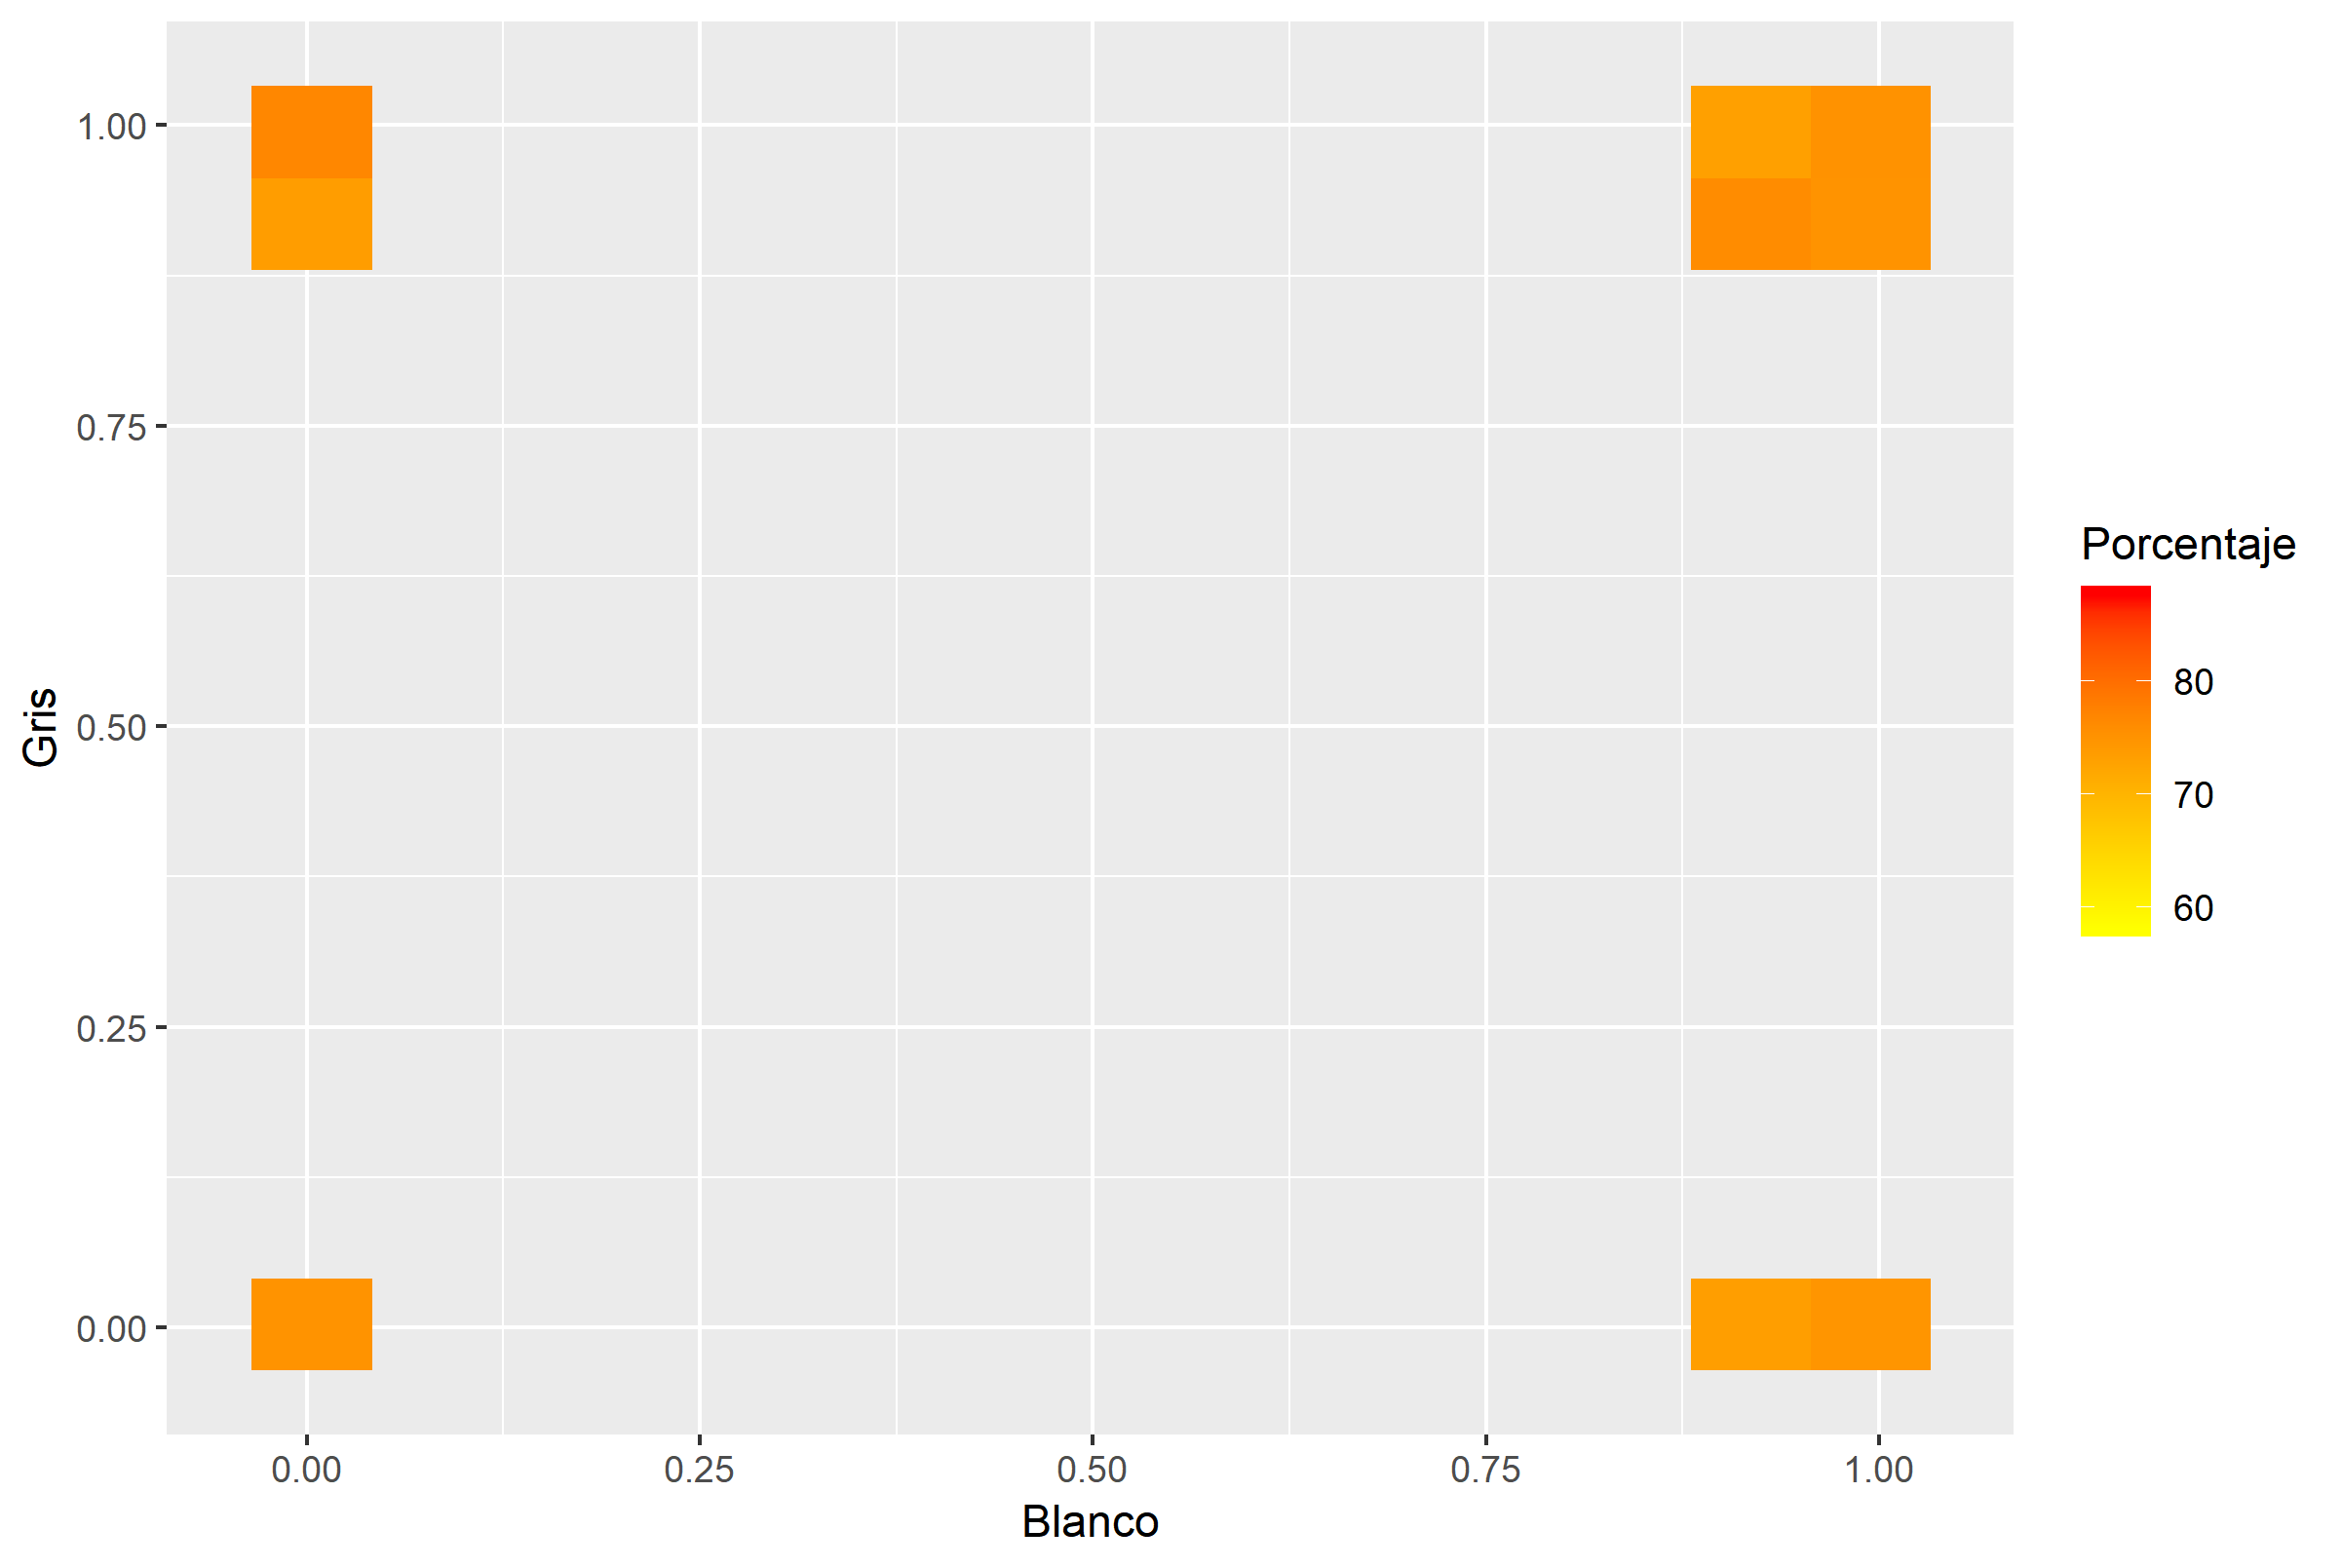
\includegraphics[width=80mm]{./plot_GB.png}}
\subfigure[]{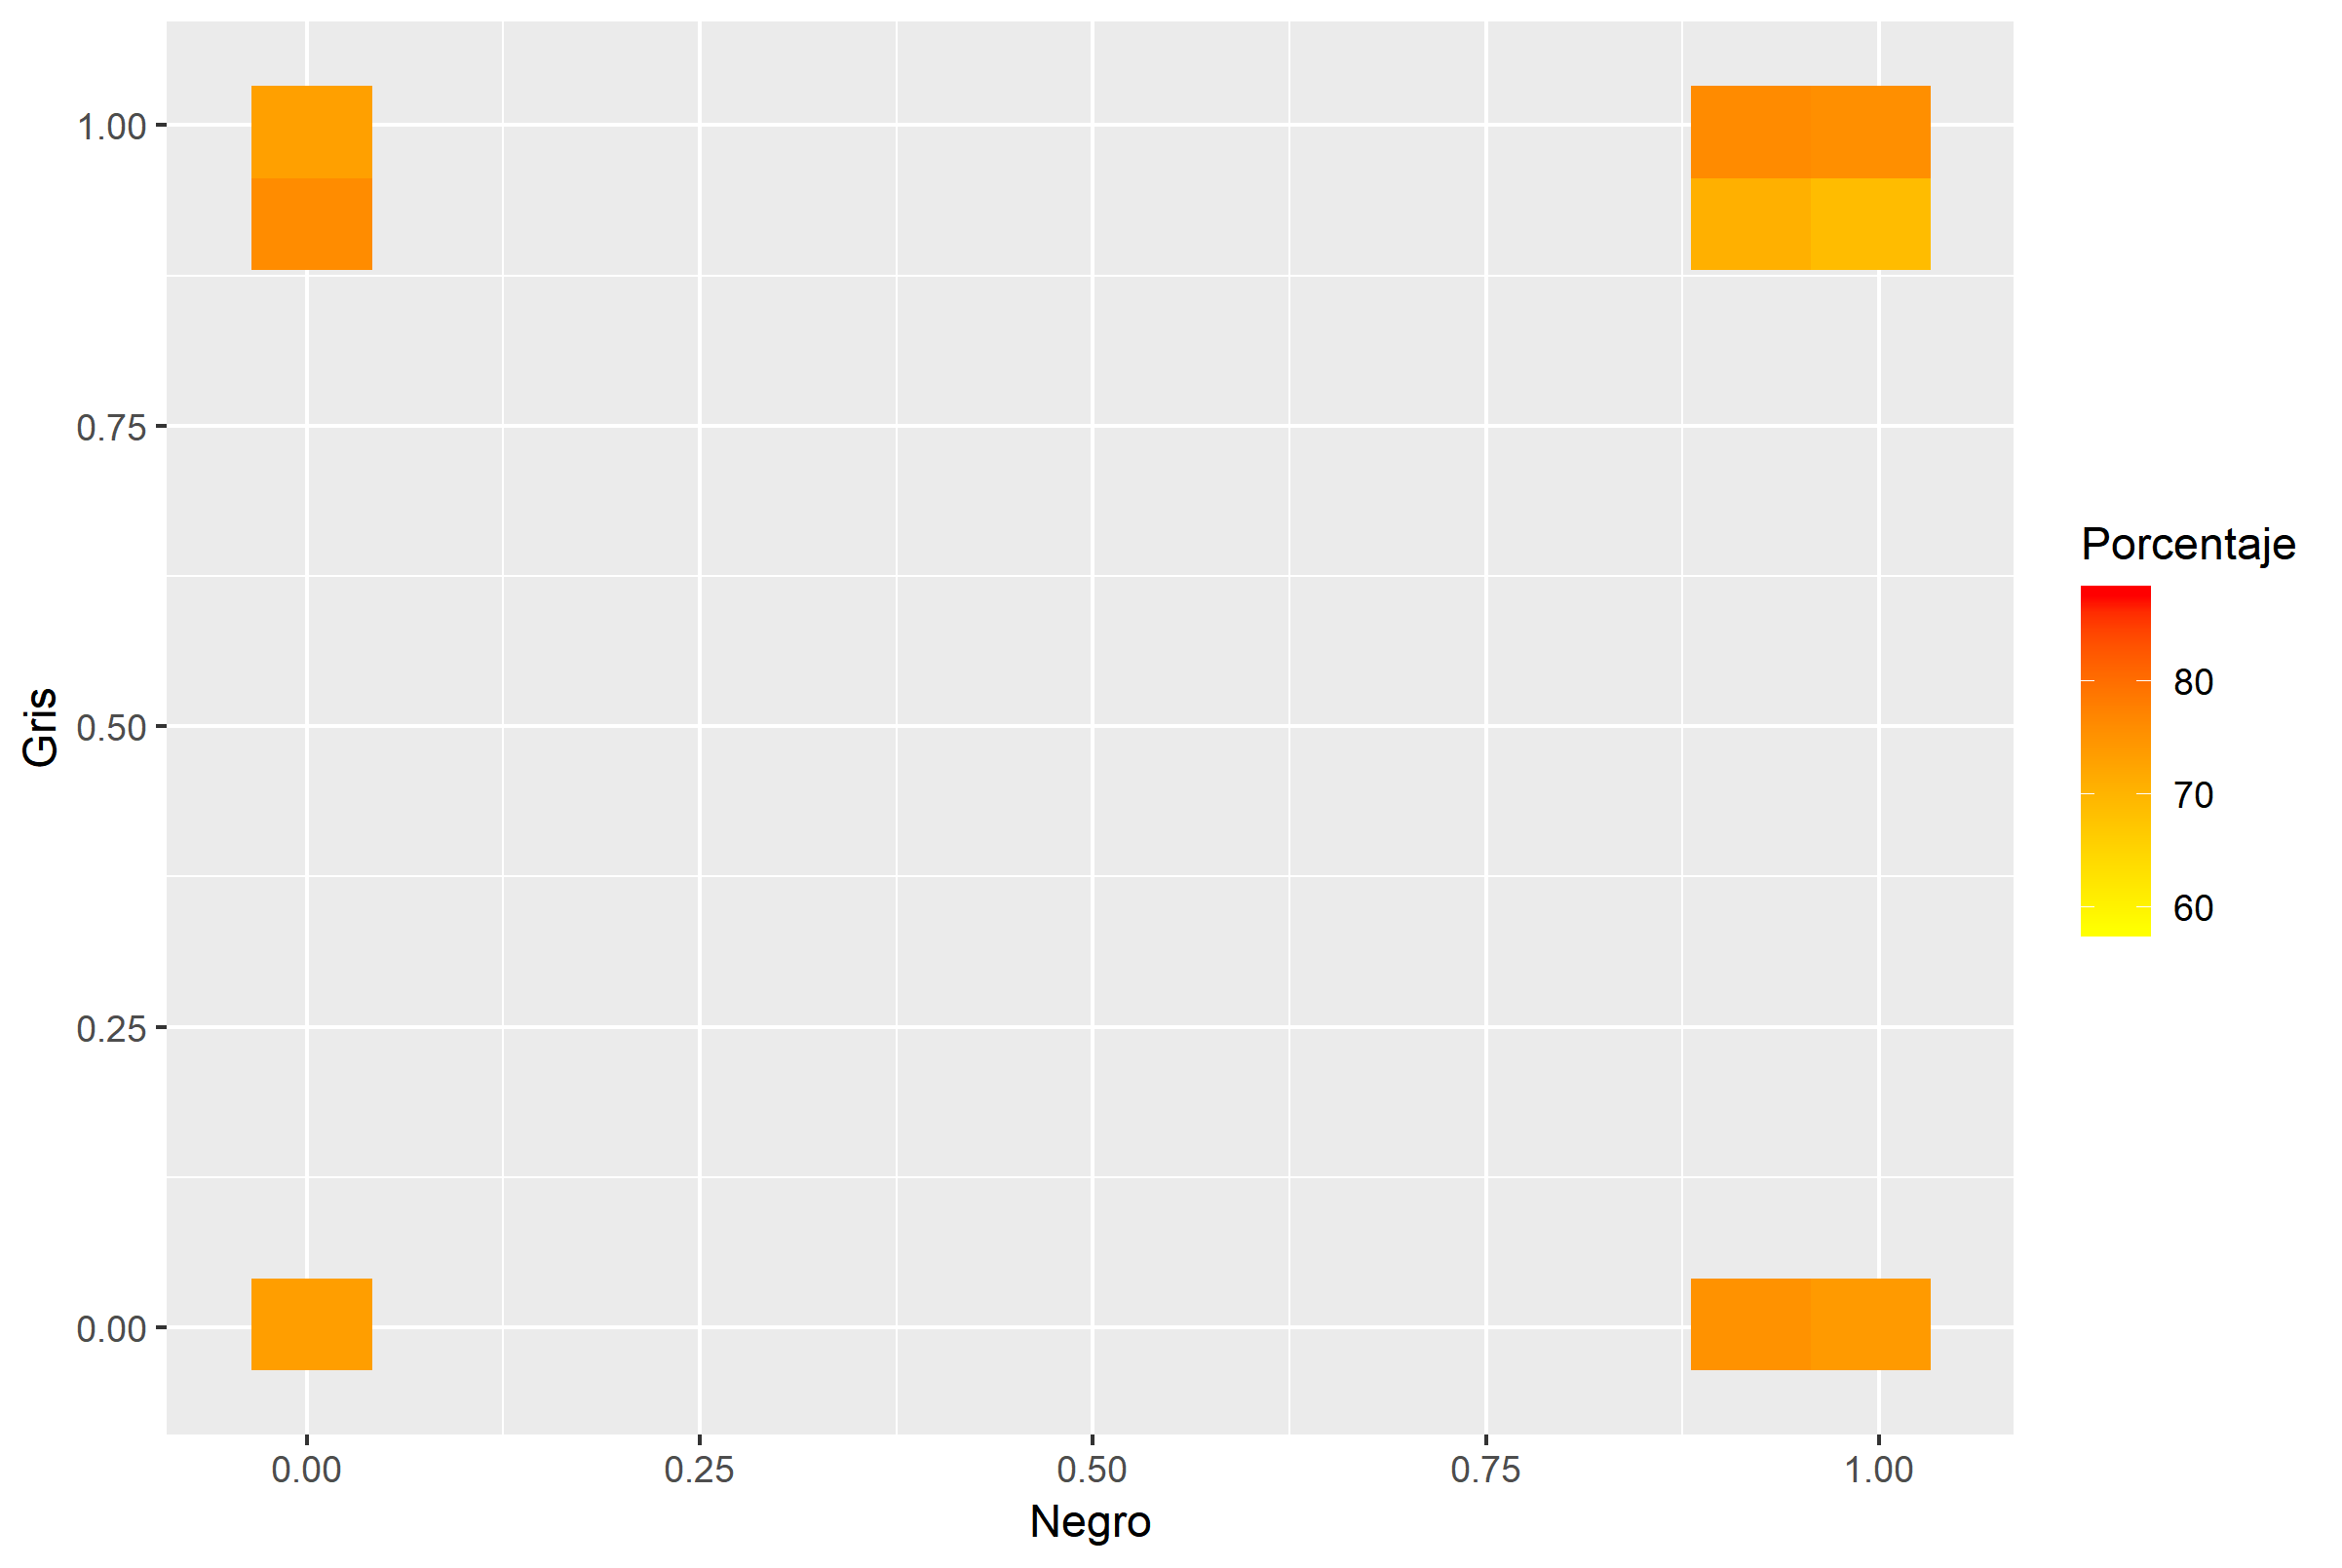
\includegraphics[width=80mm]{./plot_GN.png}}
\caption{ }\label{fig1}
\end{figure}






\newpage
\section{Conclusión}
Los pixeles que dominan la formación de caracteres son los pixeles \textit{Negro} y \textit{Gris} dado a que los porcentajes de que se reconociera correctamente los dígitos fueron mayores para estos pixeles sin importar las variaciones y combinaciones de probabilidades.

\section*{Reto 1}
El primer reto consiste en extender y entrenar la red neuronal para que reconozca además por lo menos doce símbolos ASCII adicionales, aumentando la resolución de las imágenes a $5\times 7$ de lo original de $3\times 5$, estos se obtuvieron tomando de referencia a \textit{Saus} \cite{saus}

\begin{lstlisting}[language=R]
modelos <- read.csv("digitos.reto.csv", sep=" ", header=FALSE, stringsAsFactors=F)
modelos[modelos=='n'] <- 0.995 # pixeles negros en plantillas
modelos[modelos=='g'] <- 0.92 # pixeles grises en plantillas
modelos[modelos=='b'] <- 0.002 # pixeles blancos en plantillas

r <- 7
c <- 5
dim <- r * c

n <- 49
w <- ceiling(sqrt(n))
h <- ceiling(n / w)

letras <- c(0:9, "L", "I", "C", "H", "T", "E", "F", "U", "P", "A", "W", "M")

png("plantilla.png", width=1600, height=2000)
par(mfrow=c(w, h), mar = c(0,0,7,0))
suppressMessages(library("sna"))

for (j in 1:n) {
  d <- sample(0:21, 1)
  pixeles <- runif(dim) < modelos[d + 1,] # fila 1 contiene el cero, etc.
  imagen <- matrix(pixeles, nrow=r, ncol=c, byrow=TRUE)
  plot.sociomatrix(imagen, drawlab=FALSE, diaglab=FALSE, 
                   main=paste(letras[d+1], ""), cex.main=5)
}
graphics.off()
\end{lstlisting}

\section{Resultados}
 
En la figura \ref{fig2} se observan los números y letras codificadas donde solo 18 caracteres fueron reconocidos de manera satisfactoria.

\begin{figure}[!h]
\centering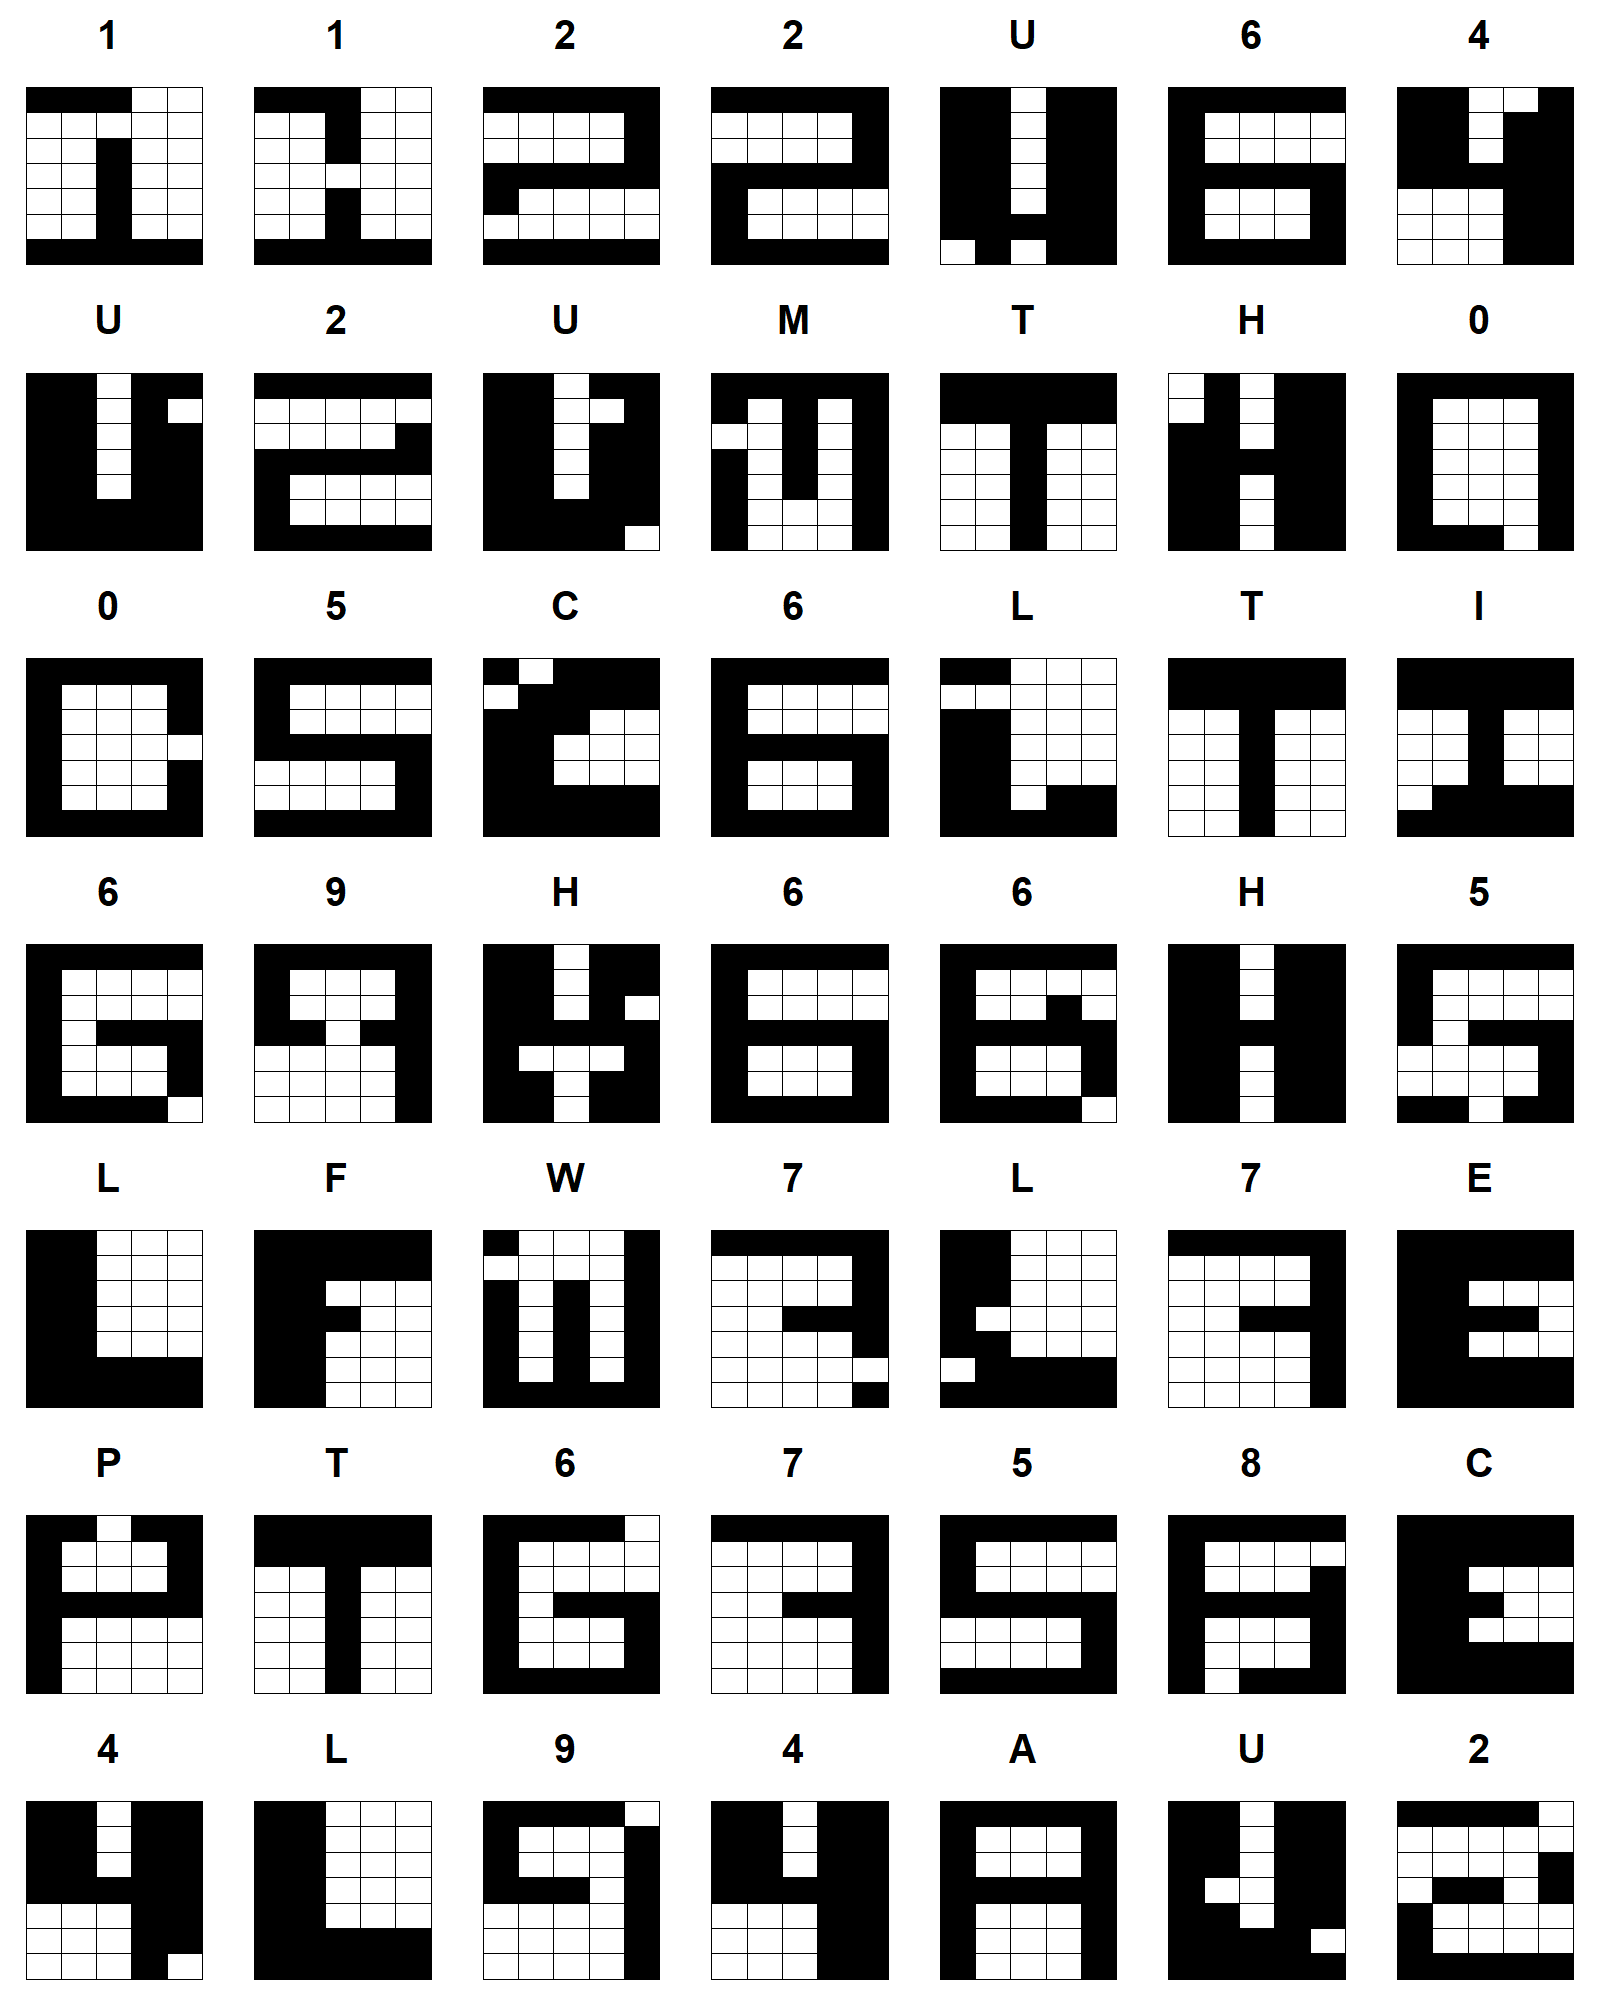
\includegraphics[width=100mm]{plantilla.png}
\caption{Caracteres de red neuronal extendida}
\label{fig2}
\end{figure}

\newpage

\section{Conclusión}
En este caso no se pudo entrenar debidamente la red neuronal bajo estas nuevas condiciones, observando la figura \ref{fig2} se puede deducir que para una red neuronal extendida se necesita mayor tiempo de entrenamiento para que posteriormente pueda hacer un reconocimiento correcto.

\newpage
\bibliographystyle{plainnat}
\bibliography{biblio}

\end{document}